% Created by tikzDevice version 0.12.6 on 2026-07-06 23:55:43
% !TEX encoding = UTF-8 Unicode
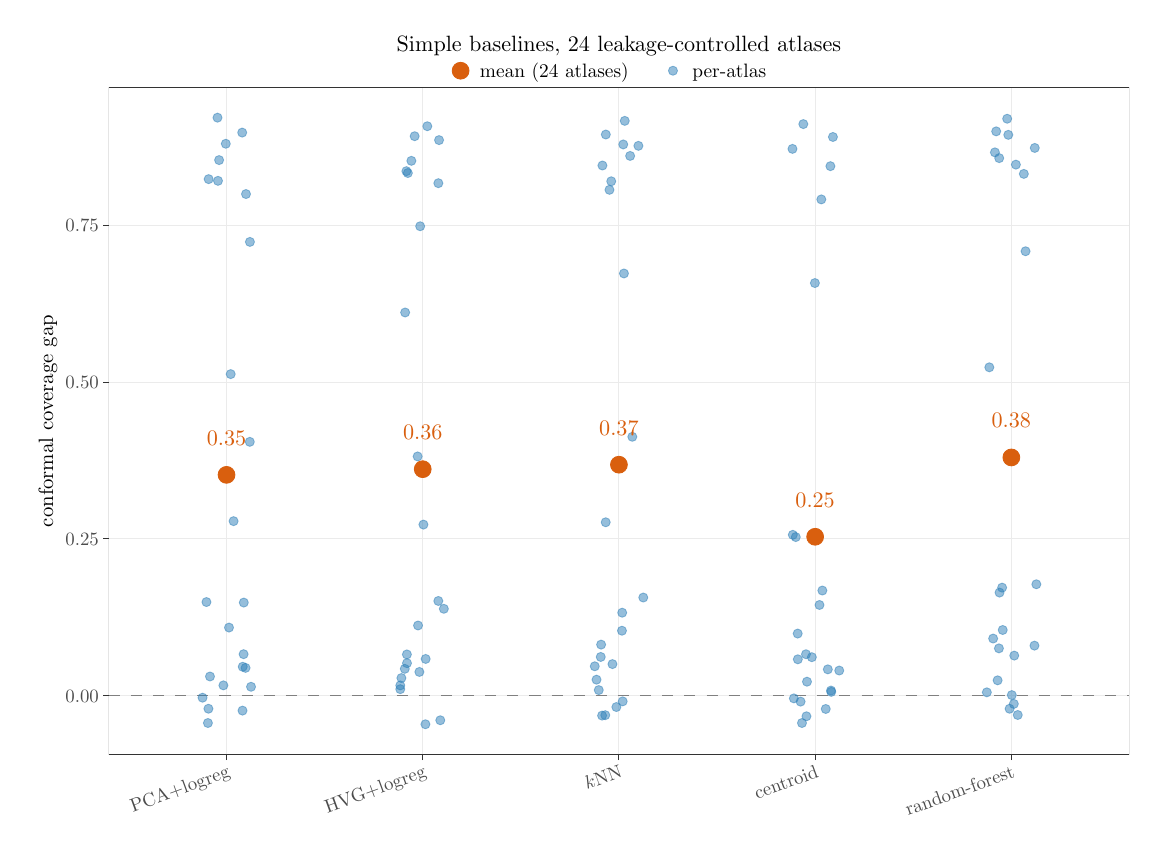
\begin{tikzpicture}[x=1pt,y=1pt]
\definecolor{fillColor}{RGB}{255,255,255}
\path[use as bounding box,fill=fillColor,fill opacity=0.00] (0,0) rectangle (403.99,289.08);
\begin{scope}
\path[clip] (  0.00,  0.00) rectangle (403.99,289.08);
\definecolor{drawColor}{RGB}{255,255,255}
\definecolor{fillColor}{RGB}{255,255,255}

\path[draw=drawColor,line width= 0.4pt,line join=round,line cap=round,fill=fillColor] (  0.00,  0.00) rectangle (403.99,289.08);
\end{scope}
\begin{scope}
\path[clip] ( 29.31, 26.41) rectangle (397.99,267.52);
\definecolor{fillColor}{RGB}{255,255,255}

\path[fill=fillColor] ( 29.31, 26.41) rectangle (397.99,267.52);
\definecolor{drawColor}{gray}{0.92}

\path[draw=drawColor,line width= 0.4pt,line join=round] ( 29.31, 47.67) --
	(397.99, 47.67);

\path[draw=drawColor,line width= 0.4pt,line join=round] ( 29.31,104.34) --
	(397.99,104.34);

\path[draw=drawColor,line width= 0.4pt,line join=round] ( 29.31,161.00) --
	(397.99,161.00);

\path[draw=drawColor,line width= 0.4pt,line join=round] ( 29.31,217.67) --
	(397.99,217.67);

\path[draw=drawColor,line width= 0.4pt,line join=round] ( 71.85, 26.41) --
	( 71.85,267.52);

\path[draw=drawColor,line width= 0.4pt,line join=round] (142.75, 26.41) --
	(142.75,267.52);

\path[draw=drawColor,line width= 0.4pt,line join=round] (213.65, 26.41) --
	(213.65,267.52);

\path[draw=drawColor,line width= 0.4pt,line join=round] (284.55, 26.41) --
	(284.55,267.52);

\path[draw=drawColor,line width= 0.4pt,line join=round] (355.45, 26.41) --
	(355.45,267.52);
\definecolor{drawColor}{gray}{0.50}

\path[draw=drawColor,line width= 0.4pt,dash pattern=on 4pt off 4pt ,line join=round] ( 29.31, 47.67) -- (397.99, 47.67);
\definecolor{drawColor}{RGB}{44,127,184}
\definecolor{fillColor}{RGB}{44,127,184}

\path[draw=drawColor,draw opacity=0.50,line width= 0.3pt,line join=round,line cap=round,fill=fillColor,fill opacity=0.50] ( 69.17,241.23) circle (  1.65);

\path[draw=drawColor,draw opacity=0.50,line width= 0.3pt,line join=round,line cap=round,fill=fillColor,fill opacity=0.50] (138.65,240.96) circle (  1.65);

\path[draw=drawColor,draw opacity=0.50,line width= 0.3pt,line join=round,line cap=round,fill=fillColor,fill opacity=0.50] (217.70,242.73) circle (  1.65);

\path[draw=drawColor,draw opacity=0.50,line width= 0.3pt,line join=round,line cap=round,fill=fillColor,fill opacity=0.50] (286.78,227.02) circle (  1.65);

\path[draw=drawColor,draw opacity=0.50,line width= 0.3pt,line join=round,line cap=round,fill=fillColor,fill opacity=0.50] (349.51,244.02) circle (  1.65);

\path[draw=drawColor,draw opacity=0.50,line width= 0.3pt,line join=round,line cap=round,fill=fillColor,fill opacity=0.50] ( 68.77,233.73) circle (  1.65);

\path[draw=drawColor,draw opacity=0.50,line width= 0.3pt,line join=round,line cap=round,fill=fillColor,fill opacity=0.50] (136.85,237.23) circle (  1.65);

\path[draw=drawColor,draw opacity=0.50,line width= 0.3pt,line join=round,line cap=round,fill=fillColor,fill opacity=0.50] (207.69,239.27) circle (  1.65);

\path[draw=drawColor,draw opacity=0.50,line width= 0.3pt,line join=round,line cap=round,fill=fillColor,fill opacity=0.50] (290.07,239.03) circle (  1.65);

\path[draw=drawColor,draw opacity=0.50,line width= 0.3pt,line join=round,line cap=round,fill=fillColor,fill opacity=0.50] (359.96,236.24) circle (  1.65);

\path[draw=drawColor,draw opacity=0.50,line width= 0.3pt,line join=round,line cap=round,fill=fillColor,fill opacity=0.50] ( 73.36,163.89) circle (  1.65);

\path[draw=drawColor,draw opacity=0.50,line width= 0.3pt,line join=round,line cap=round,fill=fillColor,fill opacity=0.50] (136.40,186.16) circle (  1.65);

\path[draw=drawColor,draw opacity=0.50,line width= 0.3pt,line join=round,line cap=round,fill=fillColor,fill opacity=0.50] (215.46,200.26) circle (  1.65);

\path[draw=drawColor,draw opacity=0.50,line width= 0.3pt,line join=round,line cap=round,fill=fillColor,fill opacity=0.50] (281.24, 62.67) circle (  1.65);

\path[draw=drawColor,draw opacity=0.50,line width= 0.3pt,line join=round,line cap=round,fill=fillColor,fill opacity=0.50] (360.58,208.29) circle (  1.65);

\path[draw=drawColor,draw opacity=0.50,line width= 0.3pt,line join=round,line cap=round,fill=fillColor,fill opacity=0.50] ( 77.63, 42.30) circle (  1.65);

\path[draw=drawColor,draw opacity=0.50,line width= 0.3pt,line join=round,line cap=round,fill=fillColor,fill opacity=0.50] (149.10, 38.81) circle (  1.65);

\path[draw=drawColor,draw opacity=0.50,line width= 0.3pt,line join=round,line cap=round,fill=fillColor,fill opacity=0.50] (212.73, 43.59) circle (  1.65);

\path[draw=drawColor,draw opacity=0.50,line width= 0.3pt,line join=round,line cap=round,fill=fillColor,fill opacity=0.50] (279.79, 37.82) circle (  1.65);

\path[draw=drawColor,draw opacity=0.50,line width= 0.3pt,line join=round,line cap=round,fill=fillColor,fill opacity=0.50] (354.81, 42.97) circle (  1.65);

\path[draw=drawColor,draw opacity=0.50,line width= 0.3pt,line join=round,line cap=round,fill=fillColor,fill opacity=0.50] ( 80.71, 50.91) circle (  1.65);

\path[draw=drawColor,draw opacity=0.50,line width= 0.3pt,line join=round,line cap=round,fill=fillColor,fill opacity=0.50] (141.55, 56.27) circle (  1.65);

\path[draw=drawColor,draw opacity=0.50,line width= 0.3pt,line join=round,line cap=round,fill=fillColor,fill opacity=0.50] (207.08, 61.69) circle (  1.65);

\path[draw=drawColor,draw opacity=0.50,line width= 0.3pt,line join=round,line cap=round,fill=fillColor,fill opacity=0.50] (293.26, 56.78) circle (  1.65);

\path[draw=drawColor,draw opacity=0.50,line width= 0.3pt,line join=round,line cap=round,fill=fillColor,fill opacity=0.50] (352.33, 71.43) circle (  1.65);

\path[draw=drawColor,draw opacity=0.50,line width= 0.3pt,line join=round,line cap=round,fill=fillColor,fill opacity=0.50] ( 77.52,251.17) circle (  1.65);

\path[draw=drawColor,draw opacity=0.50,line width= 0.3pt,line join=round,line cap=round,fill=fillColor,fill opacity=0.50] (139.83,249.86) circle (  1.65);

\path[draw=drawColor,draw opacity=0.50,line width= 0.3pt,line join=round,line cap=round,fill=fillColor,fill opacity=0.50] (208.91,250.47) circle (  1.65);

\path[draw=drawColor,draw opacity=0.50,line width= 0.3pt,line join=round,line cap=round,fill=fillColor,fill opacity=0.50] (276.36,245.28) circle (  1.65);

\path[draw=drawColor,draw opacity=0.50,line width= 0.3pt,line join=round,line cap=round,fill=fillColor,fill opacity=0.50] (349.97,251.61) circle (  1.65);

\path[draw=drawColor,draw opacity=0.50,line width= 0.3pt,line join=round,line cap=round,fill=fillColor,fill opacity=0.50] ( 80.26,139.42) circle (  1.65);

\path[draw=drawColor,draw opacity=0.50,line width= 0.3pt,line join=round,line cap=round,fill=fillColor,fill opacity=0.50] (140.91,134.14) circle (  1.65);

\path[draw=drawColor,draw opacity=0.50,line width= 0.3pt,line join=round,line cap=round,fill=fillColor,fill opacity=0.50] (218.49,141.24) circle (  1.65);

\path[draw=drawColor,draw opacity=0.50,line width= 0.3pt,line join=round,line cap=round,fill=fillColor,fill opacity=0.50] (277.55,105.01) circle (  1.65);

\path[draw=drawColor,draw opacity=0.50,line width= 0.3pt,line join=round,line cap=round,fill=fillColor,fill opacity=0.50] (347.49,166.35) circle (  1.65);

\path[draw=drawColor,draw opacity=0.50,line width= 0.3pt,line join=round,line cap=round,fill=fillColor,fill opacity=0.50] ( 71.59,247.13) circle (  1.65);

\path[draw=drawColor,draw opacity=0.50,line width= 0.3pt,line join=round,line cap=round,fill=fillColor,fill opacity=0.50] (148.65,248.45) circle (  1.65);

\path[draw=drawColor,draw opacity=0.50,line width= 0.3pt,line join=round,line cap=round,fill=fillColor,fill opacity=0.50] (220.69,246.38) circle (  1.65);

\path[draw=drawColor,draw opacity=0.50,line width= 0.3pt,line join=round,line cap=round,fill=fillColor,fill opacity=0.50] (290.98,249.58) circle (  1.65);

\path[draw=drawColor,draw opacity=0.50,line width= 0.3pt,line join=round,line cap=round,fill=fillColor,fill opacity=0.50] (363.91,245.62) circle (  1.65);

\path[draw=drawColor,draw opacity=0.50,line width= 0.3pt,line join=round,line cap=round,fill=fillColor,fill opacity=0.50] ( 70.73, 51.42) circle (  1.65);

\path[draw=drawColor,draw opacity=0.50,line width= 0.3pt,line join=round,line cap=round,fill=fillColor,fill opacity=0.50] (143.01,109.52) circle (  1.65);

\path[draw=drawColor,draw opacity=0.50,line width= 0.3pt,line join=round,line cap=round,fill=fillColor,fill opacity=0.50] (208.87,110.35) circle (  1.65);

\path[draw=drawColor,draw opacity=0.50,line width= 0.3pt,line join=round,line cap=round,fill=fillColor,fill opacity=0.50] (287.16, 85.69) circle (  1.65);

\path[draw=drawColor,draw opacity=0.50,line width= 0.3pt,line join=round,line cap=round,fill=fillColor,fill opacity=0.50] (352.11, 86.74) circle (  1.65);

\path[draw=drawColor,draw opacity=0.50,line width= 0.3pt,line join=round,line cap=round,fill=fillColor,fill opacity=0.50] ( 78.09, 81.34) circle (  1.65);

\path[draw=drawColor,draw opacity=0.50,line width= 0.3pt,line join=round,line cap=round,fill=fillColor,fill opacity=0.50] (148.39, 81.92) circle (  1.65);

\path[draw=drawColor,draw opacity=0.50,line width= 0.3pt,line join=round,line cap=round,fill=fillColor,fill opacity=0.50] (214.83, 77.68) circle (  1.65);

\path[draw=drawColor,draw opacity=0.50,line width= 0.3pt,line join=round,line cap=round,fill=fillColor,fill opacity=0.50] (286.12, 80.47) circle (  1.65);

\path[draw=drawColor,draw opacity=0.50,line width= 0.3pt,line join=round,line cap=round,fill=fillColor,fill opacity=0.50] (364.48, 87.95) circle (  1.65);

\path[draw=drawColor,draw opacity=0.50,line width= 0.3pt,line join=round,line cap=round,fill=fillColor,fill opacity=0.50] ( 65.13, 37.82) circle (  1.65);

\path[draw=drawColor,draw opacity=0.50,line width= 0.3pt,line join=round,line cap=round,fill=fillColor,fill opacity=0.50] (143.73, 37.37) circle (  1.65);

\path[draw=drawColor,draw opacity=0.50,line width= 0.3pt,line join=round,line cap=round,fill=fillColor,fill opacity=0.50] (207.56, 40.50) circle (  1.65);

\path[draw=drawColor,draw opacity=0.50,line width= 0.3pt,line join=round,line cap=round,fill=fillColor,fill opacity=0.50] (276.86, 46.72) circle (  1.65);

\path[draw=drawColor,draw opacity=0.50,line width= 0.3pt,line join=round,line cap=round,fill=fillColor,fill opacity=0.50] (357.76, 40.72) circle (  1.65);

\path[draw=drawColor,draw opacity=0.50,line width= 0.3pt,line join=round,line cap=round,fill=fillColor,fill opacity=0.50] ( 64.60, 81.53) circle (  1.65);

\path[draw=drawColor,draw opacity=0.50,line width= 0.3pt,line join=round,line cap=round,fill=fillColor,fill opacity=0.50] (150.38, 79.09) circle (  1.65);

\path[draw=drawColor,draw opacity=0.50,line width= 0.3pt,line join=round,line cap=round,fill=fillColor,fill opacity=0.50] (211.31, 59.11) circle (  1.65);

\path[draw=drawColor,draw opacity=0.50,line width= 0.3pt,line join=round,line cap=round,fill=fillColor,fill opacity=0.50] (289.13, 57.21) circle (  1.65);

\path[draw=drawColor,draw opacity=0.50,line width= 0.3pt,line join=round,line cap=round,fill=fillColor,fill opacity=0.50] (363.80, 65.78) circle (  1.65);

\path[draw=drawColor,draw opacity=0.50,line width= 0.3pt,line join=round,line cap=round,fill=fillColor,fill opacity=0.50] ( 68.59,256.56) circle (  1.65);

\path[draw=drawColor,draw opacity=0.50,line width= 0.3pt,line join=round,line cap=round,fill=fillColor,fill opacity=0.50] (144.41,253.46) circle (  1.65);

\path[draw=drawColor,draw opacity=0.50,line width= 0.3pt,line join=round,line cap=round,fill=fillColor,fill opacity=0.50] (215.75,255.40) circle (  1.65);

\path[draw=drawColor,draw opacity=0.50,line width= 0.3pt,line join=round,line cap=round,fill=fillColor,fill opacity=0.50] (280.28,254.24) circle (  1.65);

\path[draw=drawColor,draw opacity=0.50,line width= 0.3pt,line join=round,line cap=round,fill=fillColor,fill opacity=0.50] (353.94,256.17) circle (  1.65);

\path[draw=drawColor,draw opacity=0.50,line width= 0.3pt,line join=round,line cap=round,fill=fillColor,fill opacity=0.50] ( 74.40,110.76) circle (  1.65);

\path[draw=drawColor,draw opacity=0.50,line width= 0.3pt,line join=round,line cap=round,fill=fillColor,fill opacity=0.50] (136.27, 57.40) circle (  1.65);

\path[draw=drawColor,draw opacity=0.50,line width= 0.3pt,line join=round,line cap=round,fill=fillColor,fill opacity=0.50] (207.21, 66.15) circle (  1.65);

\path[draw=drawColor,draw opacity=0.50,line width= 0.3pt,line join=round,line cap=round,fill=fillColor,fill opacity=0.50] (276.48,105.82) circle (  1.65);

\path[draw=drawColor,draw opacity=0.50,line width= 0.3pt,line join=round,line cap=round,fill=fillColor,fill opacity=0.50] (351.18, 84.95) circle (  1.65);

\path[draw=drawColor,draw opacity=0.50,line width= 0.3pt,line join=round,line cap=round,fill=fillColor,fill opacity=0.50] ( 63.19, 46.97) circle (  1.65);

\path[draw=drawColor,draw opacity=0.50,line width= 0.3pt,line join=round,line cap=round,fill=fillColor,fill opacity=0.50] (134.64, 51.40) circle (  1.65);

\path[draw=drawColor,draw opacity=0.50,line width= 0.3pt,line join=round,line cap=round,fill=fillColor,fill opacity=0.50] (215.00, 45.64) circle (  1.65);

\path[draw=drawColor,draw opacity=0.50,line width= 0.3pt,line join=round,line cap=round,fill=fillColor,fill opacity=0.50] (279.29, 45.55) circle (  1.65);

\path[draw=drawColor,draw opacity=0.50,line width= 0.3pt,line join=round,line cap=round,fill=fillColor,fill opacity=0.50] (346.59, 48.90) circle (  1.65);

\path[draw=drawColor,draw opacity=0.50,line width= 0.3pt,line join=round,line cap=round,fill=fillColor,fill opacity=0.50] ( 65.32, 42.98) circle (  1.65);

\path[draw=drawColor,draw opacity=0.50,line width= 0.3pt,line join=round,line cap=round,fill=fillColor,fill opacity=0.50] (134.64, 50.05) circle (  1.65);

\path[draw=drawColor,draw opacity=0.50,line width= 0.3pt,line join=round,line cap=round,fill=fillColor,fill opacity=0.50] (206.36, 49.72) circle (  1.65);

\path[draw=drawColor,draw opacity=0.50,line width= 0.3pt,line join=round,line cap=round,fill=fillColor,fill opacity=0.50] (290.38, 49.07) circle (  1.65);

\path[draw=drawColor,draw opacity=0.50,line width= 0.3pt,line join=round,line cap=round,fill=fillColor,fill opacity=0.50] (355.61, 47.91) circle (  1.65);

\path[draw=drawColor,draw opacity=0.50,line width= 0.3pt,line join=round,line cap=round,fill=fillColor,fill opacity=0.50] ( 78.89,228.96) circle (  1.65);

\path[draw=drawColor,draw opacity=0.50,line width= 0.3pt,line join=round,line cap=round,fill=fillColor,fill opacity=0.50] (148.40,232.88) circle (  1.65);

\path[draw=drawColor,draw opacity=0.50,line width= 0.3pt,line join=round,line cap=round,fill=fillColor,fill opacity=0.50] (210.23,230.48) circle (  1.65);

\path[draw=drawColor,draw opacity=0.50,line width= 0.3pt,line join=round,line cap=round,fill=fillColor,fill opacity=0.50] (278.24, 70.14) circle (  1.65);

\path[draw=drawColor,draw opacity=0.50,line width= 0.3pt,line join=round,line cap=round,fill=fillColor,fill opacity=0.50] (357.09,239.59) circle (  1.65);

\path[draw=drawColor,draw opacity=0.50,line width= 0.3pt,line join=round,line cap=round,fill=fillColor,fill opacity=0.50] ( 72.75, 72.31) circle (  1.65);

\path[draw=drawColor,draw opacity=0.50,line width= 0.3pt,line join=round,line cap=round,fill=fillColor,fill opacity=0.50] (141.06, 73.06) circle (  1.65);

\path[draw=drawColor,draw opacity=0.50,line width= 0.3pt,line join=round,line cap=round,fill=fillColor,fill opacity=0.50] (222.45, 83.16) circle (  1.65);

\path[draw=drawColor,draw opacity=0.50,line width= 0.3pt,line join=round,line cap=round,fill=fillColor,fill opacity=0.50] (288.38, 42.89) circle (  1.65);

\path[draw=drawColor,draw opacity=0.50,line width= 0.3pt,line join=round,line cap=round,fill=fillColor,fill opacity=0.50] (350.96, 64.79) circle (  1.65);

\path[draw=drawColor,draw opacity=0.50,line width= 0.3pt,line join=round,line cap=round,fill=fillColor,fill opacity=0.50] ( 78.73, 57.74) circle (  1.65);

\path[draw=drawColor,draw opacity=0.50,line width= 0.3pt,line join=round,line cap=round,fill=fillColor,fill opacity=0.50] (137.06, 59.44) circle (  1.65);

\path[draw=drawColor,draw opacity=0.50,line width= 0.3pt,line join=round,line cap=round,fill=fillColor,fill opacity=0.50] (204.91, 58.32) circle (  1.65);

\path[draw=drawColor,draw opacity=0.50,line width= 0.3pt,line join=round,line cap=round,fill=fillColor,fill opacity=0.50] (283.36, 61.60) circle (  1.65);

\path[draw=drawColor,draw opacity=0.50,line width= 0.3pt,line join=round,line cap=round,fill=fillColor,fill opacity=0.50] (356.50, 62.18) circle (  1.65);

\path[draw=drawColor,draw opacity=0.50,line width= 0.3pt,line join=round,line cap=round,fill=fillColor,fill opacity=0.50] ( 80.31,211.66) circle (  1.65);

\path[draw=drawColor,draw opacity=0.50,line width= 0.3pt,line join=round,line cap=round,fill=fillColor,fill opacity=0.50] (141.83,217.32) circle (  1.65);

\path[draw=drawColor,draw opacity=0.50,line width= 0.3pt,line join=round,line cap=round,fill=fillColor,fill opacity=0.50] (210.87,233.57) circle (  1.65);

\path[draw=drawColor,draw opacity=0.50,line width= 0.3pt,line join=round,line cap=round,fill=fillColor,fill opacity=0.50] (284.46,196.80) circle (  1.65);

\path[draw=drawColor,draw opacity=0.50,line width= 0.3pt,line join=round,line cap=round,fill=fillColor,fill opacity=0.50] (351.06,241.94) circle (  1.65);

\path[draw=drawColor,draw opacity=0.50,line width= 0.3pt,line join=round,line cap=round,fill=fillColor,fill opacity=0.50] ( 78.02, 62.69) circle (  1.65);

\path[draw=drawColor,draw opacity=0.50,line width= 0.3pt,line join=round,line cap=round,fill=fillColor,fill opacity=0.50] (143.81, 60.97) circle (  1.65);

\path[draw=drawColor,draw opacity=0.50,line width= 0.3pt,line join=round,line cap=round,fill=fillColor,fill opacity=0.50] (205.55, 53.48) circle (  1.65);

\path[draw=drawColor,draw opacity=0.50,line width= 0.3pt,line join=round,line cap=round,fill=fillColor,fill opacity=0.50] (281.60, 52.75) circle (  1.65);

\path[draw=drawColor,draw opacity=0.50,line width= 0.3pt,line join=round,line cap=round,fill=fillColor,fill opacity=0.50] (350.48, 53.24) circle (  1.65);

\path[draw=drawColor,draw opacity=0.50,line width= 0.3pt,line join=round,line cap=round,fill=fillColor,fill opacity=0.50] ( 77.70, 58.15) circle (  1.65);

\path[draw=drawColor,draw opacity=0.50,line width= 0.3pt,line join=round,line cap=round,fill=fillColor,fill opacity=0.50] (135.05, 54.07) circle (  1.65);

\path[draw=drawColor,draw opacity=0.50,line width= 0.3pt,line join=round,line cap=round,fill=fillColor,fill opacity=0.50] (208.72, 40.65) circle (  1.65);

\path[draw=drawColor,draw opacity=0.50,line width= 0.3pt,line join=round,line cap=round,fill=fillColor,fill opacity=0.50] (281.41, 40.25) circle (  1.65);

\path[draw=drawColor,draw opacity=0.50,line width= 0.3pt,line join=round,line cap=round,fill=fillColor,fill opacity=0.50] (356.34, 44.72) circle (  1.65);

\path[draw=drawColor,draw opacity=0.50,line width= 0.3pt,line join=round,line cap=round,fill=fillColor,fill opacity=0.50] ( 65.88, 54.63) circle (  1.65);

\path[draw=drawColor,draw opacity=0.50,line width= 0.3pt,line join=round,line cap=round,fill=fillColor,fill opacity=0.50] (137.03, 62.60) circle (  1.65);

\path[draw=drawColor,draw opacity=0.50,line width= 0.3pt,line join=round,line cap=round,fill=fillColor,fill opacity=0.50] (214.74, 71.17) circle (  1.65);

\path[draw=drawColor,draw opacity=0.50,line width= 0.3pt,line join=round,line cap=round,fill=fillColor,fill opacity=0.50] (278.29, 60.84) circle (  1.65);

\path[draw=drawColor,draw opacity=0.50,line width= 0.3pt,line join=round,line cap=round,fill=fillColor,fill opacity=0.50] (348.87, 68.34) circle (  1.65);

\path[draw=drawColor,draw opacity=0.50,line width= 0.3pt,line join=round,line cap=round,fill=fillColor,fill opacity=0.50] ( 65.39,234.35) circle (  1.65);

\path[draw=drawColor,draw opacity=0.50,line width= 0.3pt,line join=round,line cap=round,fill=fillColor,fill opacity=0.50] (137.37,236.55) circle (  1.65);

\path[draw=drawColor,draw opacity=0.50,line width= 0.3pt,line join=round,line cap=round,fill=fillColor,fill opacity=0.50] (215.21,246.88) circle (  1.65);

\path[draw=drawColor,draw opacity=0.50,line width= 0.3pt,line join=round,line cap=round,fill=fillColor,fill opacity=0.50] (290.28, 49.55) circle (  1.65);

\path[draw=drawColor,draw opacity=0.50,line width= 0.3pt,line join=round,line cap=round,fill=fillColor,fill opacity=0.50] (354.35,250.35) circle (  1.65);
\definecolor{drawColor}{RGB}{217,95,14}
\definecolor{fillColor}{RGB}{217,95,14}

\path[draw=drawColor,line width= 0.3pt,line join=round,line cap=round,fill=fillColor] ( 71.85,127.49) circle (  3.04);

\path[draw=drawColor,line width= 0.3pt,line join=round,line cap=round,fill=fillColor] (142.75,129.54) circle (  3.04);

\path[draw=drawColor,line width= 0.3pt,line join=round,line cap=round,fill=fillColor] (213.65,131.16) circle (  3.04);

\path[draw=drawColor,line width= 0.3pt,line join=round,line cap=round,fill=fillColor] (284.55,105.12) circle (  3.04);

\path[draw=drawColor,line width= 0.3pt,line join=round,line cap=round,fill=fillColor] (355.45,133.78) circle (  3.04);

\node[text=drawColor,anchor=base,inner sep=0pt, outer sep=0pt, scale=  0.80] at ( 71.85,138.19) {0.35};

\node[text=drawColor,anchor=base,inner sep=0pt, outer sep=0pt, scale=  0.80] at (142.75,140.24) {0.36};

\node[text=drawColor,anchor=base,inner sep=0pt, outer sep=0pt, scale=  0.80] at (213.65,141.86) {0.37};

\node[text=drawColor,anchor=base,inner sep=0pt, outer sep=0pt, scale=  0.80] at (284.55,115.82) {0.25};

\node[text=drawColor,anchor=base,inner sep=0pt, outer sep=0pt, scale=  0.80] at (355.45,144.48) {0.38};
\definecolor{drawColor}{gray}{0.20}

\path[draw=drawColor,line width= 0.4pt,line join=round,line cap=round] ( 29.31, 26.41) rectangle (397.99,267.52);
\end{scope}
\begin{scope}
\path[clip] (  0.00,  0.00) rectangle (403.99,289.08);
\definecolor{drawColor}{gray}{0.30}

\node[text=drawColor,anchor=base east,inner sep=0pt, outer sep=0pt, scale=  0.68] at ( 25.71, 45.33) {0.00};

\node[text=drawColor,anchor=base east,inner sep=0pt, outer sep=0pt, scale=  0.68] at ( 25.71,101.99) {0.25};

\node[text=drawColor,anchor=base east,inner sep=0pt, outer sep=0pt, scale=  0.68] at ( 25.71,158.66) {0.50};

\node[text=drawColor,anchor=base east,inner sep=0pt, outer sep=0pt, scale=  0.68] at ( 25.71,215.33) {0.75};
\end{scope}
\begin{scope}
\path[clip] (  0.00,  0.00) rectangle (403.99,289.08);
\definecolor{drawColor}{gray}{0.20}

\path[draw=drawColor,line width= 0.4pt,line join=round] ( 27.31, 47.67) --
	( 29.31, 47.67);

\path[draw=drawColor,line width= 0.4pt,line join=round] ( 27.31,104.34) --
	( 29.31,104.34);

\path[draw=drawColor,line width= 0.4pt,line join=round] ( 27.31,161.00) --
	( 29.31,161.00);

\path[draw=drawColor,line width= 0.4pt,line join=round] ( 27.31,217.67) --
	( 29.31,217.67);
\end{scope}
\begin{scope}
\path[clip] (  0.00,  0.00) rectangle (403.99,289.08);
\definecolor{drawColor}{gray}{0.20}

\path[draw=drawColor,line width= 0.4pt,line join=round] ( 71.85, 24.41) --
	( 71.85, 26.41);

\path[draw=drawColor,line width= 0.4pt,line join=round] (142.75, 24.41) --
	(142.75, 26.41);

\path[draw=drawColor,line width= 0.4pt,line join=round] (213.65, 24.41) --
	(213.65, 26.41);

\path[draw=drawColor,line width= 0.4pt,line join=round] (284.55, 24.41) --
	(284.55, 26.41);

\path[draw=drawColor,line width= 0.4pt,line join=round] (355.45, 24.41) --
	(355.45, 26.41);
\end{scope}
\begin{scope}
\path[clip] (  0.00,  0.00) rectangle (403.99,289.08);
\definecolor{drawColor}{gray}{0.30}

\node[text=drawColor,rotate= 20.00,anchor=base east,inner sep=0pt, outer sep=0pt, scale=  0.68] at ( 73.45, 18.41) {PCA+logreg};

\node[text=drawColor,rotate= 20.00,anchor=base east,inner sep=0pt, outer sep=0pt, scale=  0.68] at (144.35, 18.41) {HVG+logreg};

\node[text=drawColor,rotate= 20.00,anchor=base east,inner sep=0pt, outer sep=0pt, scale=  0.68] at (215.25, 18.41) {$k$NN};

\node[text=drawColor,rotate= 20.00,anchor=base east,inner sep=0pt, outer sep=0pt, scale=  0.68] at (286.15, 18.41) {centroid};

\node[text=drawColor,rotate= 20.00,anchor=base east,inner sep=0pt, outer sep=0pt, scale=  0.68] at (357.05, 18.41) {random-forest};
\end{scope}
\begin{scope}
\path[clip] (  0.00,  0.00) rectangle (403.99,289.08);
\definecolor{drawColor}{RGB}{0,0,0}

\node[text=drawColor,rotate= 90.00,anchor=base,inner sep=0pt, outer sep=0pt, scale=  0.75] at (  9.17,146.96) {conformal coverage gap};
\end{scope}
\begin{scope}
\path[clip] (  0.00,  0.00) rectangle (403.99,289.08);
\definecolor{fillColor}{RGB}{255,255,255}

\path[fill=fillColor] (151.44,269.52) rectangle (275.86,277.52);
\end{scope}
\begin{scope}
\path[clip] (  0.00,  0.00) rectangle (403.99,289.08);
\definecolor{fillColor}{RGB}{255,255,255}

\path[fill=fillColor] (152.44,269.52) rectangle (160.44,277.52);
\definecolor{drawColor}{RGB}{217,95,14}
\definecolor{fillColor}{RGB}{217,95,14}

\path[draw=drawColor,line width= 0.3pt,line join=round,line cap=round,fill=fillColor] (156.44,273.52) circle (  3.04);
\end{scope}
\begin{scope}
\path[clip] (  0.00,  0.00) rectangle (403.99,289.08);
\definecolor{fillColor}{RGB}{255,255,255}

\path[fill=fillColor] (229.17,269.52) rectangle (237.17,277.52);
\definecolor{drawColor}{RGB}{44,127,184}
\definecolor{fillColor}{RGB}{44,127,184}

\path[draw=drawColor,draw opacity=0.50,line width= 0.3pt,line join=round,line cap=round,fill=fillColor,fill opacity=0.50] (233.17,273.52) circle (  1.65);
\end{scope}
\begin{scope}
\path[clip] (  0.00,  0.00) rectangle (403.99,289.08);
\definecolor{drawColor}{RGB}{0,0,0}

\node[text=drawColor,anchor=base west,inner sep=0pt, outer sep=0pt, scale=  0.70] at (163.44,271.10) {mean (24 atlases)};
\end{scope}
\begin{scope}
\path[clip] (  0.00,  0.00) rectangle (403.99,289.08);
\definecolor{drawColor}{RGB}{0,0,0}

\node[text=drawColor,anchor=base west,inner sep=0pt, outer sep=0pt, scale=  0.70] at (240.17,271.10) {per-atlas};
\end{scope}
\begin{scope}
\path[clip] (  0.00,  0.00) rectangle (403.99,289.08);
\definecolor{drawColor}{RGB}{0,0,0}

\node[text=drawColor,anchor=base,inner sep=0pt, outer sep=0pt, scale=  0.80] at (213.65,280.57) {Simple baselines, 24 leakage-controlled atlases};
\end{scope}
\end{tikzpicture}
